\documentclass[final]{beamer}

% ====================
% Packages
% ====================

\usepackage[T1]{fontenc}
\usepackage{lmodern}
\usepackage[size=custom,width=120,height=72,scale=1.0]{beamerposter}
\usetheme{gemini}
\usecolortheme{uchicago}
\usepackage{graphicx}
\usepackage{booktabs}
\usepackage{tikz}
\usepackage{float}
\usepackage{caption}
\usepackage{subcaption}
\usepackage{subfigure}
\usepackage{pgfplots}
\pgfplotsset{compat=1.17}

% ====================
% Lengths
% ====================

% If you have N columns, choose \sepwidth and \colwidth such that
% (N+1)*\sepwidth + N*\colwidth = \paperwidth
\newlength{\sepwidth}
\newlength{\colwidth}
\setlength{\sepwidth}{0.025\paperwidth}
\setlength{\colwidth}{0.3\paperwidth}

\newcommand{\separatorcolumn}{\begin{column}{\sepwidth}\end{column}}

% ====================
% Title
% ====================

\title{Model of Charge Distribution for EMCCD}

\author{Marie Yau \inst{1} \and Ivan Kotov \inst{2}}

\institute[shortinst]{\inst{1} University of California, Berkeley \samelineand \inst{2} Brookhaven National Laboratory}

% ====================
% Footer (optional)
% ====================

\footercontent{
  \href{https://www.bnl.gov}{https://www.bnl.gov} \hfill
  Instrumentation Division, Brookhaven National Laboratory \hfill
  \href{mailto:yau.marie@berkeley.edu}{yau.marie@berkeley.edu}}
% (can be left out to remove footer)

% ====================
% Logo (optional)
% ====================

% use this to include logos on the left and/or right side of the header:
% \logoright{\includegraphics[height=7cm]{logo1.pdf}}
% \logoleft{\includegraphics[height=7cm]{logo2.pdf}}

% ====================
% Body
% ====================

\begin{document}
\addtobeamertemplate{headline}{}
{
    \begin{tikzpicture}[remember picture,overlay]
      \node [anchor=north west, inner sep=3cm] at ([xshift=0.0cm,yshift=1.0cm]current page.north west)
      {
\includegraphics[height=5.0cm]{images/doe.png}}; % also try shield-white.eps
      \node [anchor=north east, inner sep=3cm] at ([xshift=0.0cm,yshift=1cm]current page.north east)
      {
\includegraphics[height=5.0cm]{images/bnl.png}};
    \end{tikzpicture}
}

\begin{frame}[t]
\begin{columns}[t]
\separatorcolumn

\begin{column}{\colwidth}

  %%%%%%%%%%%%%%%%%%%%%%%%%%%%%%%%%%%%%%%%%%%%%%%%%%%%%%%%%
  %%%%%%%%%%%%%%%%%%%%%%%%%%%%%%%%%%%%%%%%%%%%%%%%%%%%%%%%%
  \begin{block}{Abstract}

    The Soft Inelastic X-ray Scattering (SIX) beamline at the National Synchrotron Light Source II located at the Brookhaven National Laboratory uses x-ray to study the composition of a material. It is done by letting the x-ray scatter over the material. The x-ray is then detected by an electron camera (EMCCD) that is composed of a pixelated grid. By measuring the charge accumulated in each pixel, the camera produces an image showing the proportion of the x-ray that was scattered over the material, enabling us to find out what its structure is. Using this method of x-ray scattering, it is possible to achieve a very high image accuracy because we can deduce the position of the x-ray with accuracy better than its pixel pitch. The goal of my project was to develop a program that calculates the exact position of the x-ray given an image. When we receive a charge distribution for an unknown original x-ray coordinate, we can fit two-dimensional Gaussian model to our distribution using the least squares method. We have estimated the model accuracy by precomputing charge values for many different x-ray positions on the detector using a mathematical formula. Since the x-ray generates a charge on the pixel it hits and its neighboring pixels, we generate a charge distribution over detector’s pixels for each x-ray position. As a result of my internship, I have developed a program that enables other scientists to study structures of various materials more accurately. During the process, I have improved my programming skills and learned to work with many optimization packages.

  \end{block}
  %%%%%%%%%%%%%%%%%%%%%%%%%%%%%%%%%%%%%%%%%%%%%%%%%%%%%%%%%
  %%%%%%%%%%%%%%%%%%%%%%%%%%%%%%%%%%%%%%%%%%%%%%%%%%%%%%%%%

  
  %%%%%%%%%%%%%%%%%%%%%%%%%%%%%%%%%%%%%%%%%%%%%%%%%%%%%%%%%
  %%%%%%%%%%%%%%%%%%%%%%%%%%%%%%%%%%%%%%%%%%%%%%%%%%%%%%%%%
  \begin{block}{Electron Camera}
    An EMCCD camera produces a black and white pixelated image such as the one in the Figure 1. The whiter a pixel is, the more charge was detected in the pixel by the camera. Therefore, the whiter spots in the image are the spots where the x-ray hit.

    \begin{figure}[H]
        \centering
        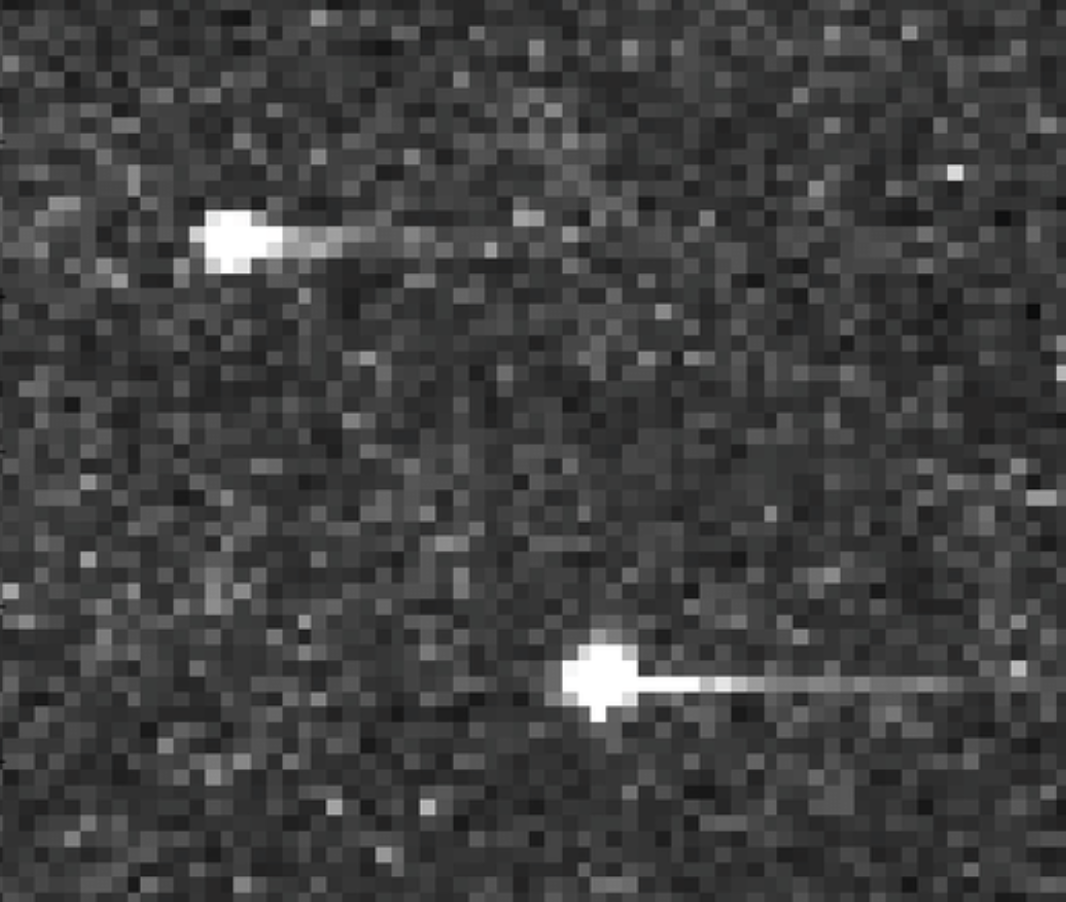
\includegraphics[width=0.6\linewidth]{images/emccd.png}
        \caption{Image produced by EMCCDs}
        \label{fig:emccd}
    \end{figure}

    The x-ray hits the pixelated grid of EMCCD at the initial point $(x_0, y_0, z_0)$. We can calculate a theoretical charge accumulated in each pixel in the grid of EMCCD using the following formula where $x = [b_i, b_{i+1}]$ and $y = [c_j, c_{j+1}]$ are pixel borders.

    \begin{equation} 
    \label{eq:q}
    q_{ij} =    
     2 \sum\limits_{n=0}^\infty 
     \alpha_n  \cdot \sin(\alpha_n z_0)
      \int \limits_{0} ^\infty    \exp \left( - \frac{\alpha_n^2}{2} \sigma^2 \right) 
      \frac{1}{\pi}  \int \limits_{b_i} ^{b_{i+1}}  \int \limits_{c_j} ^{c_{j+1}}   
      \exp \left(  - \frac{r^2}{2 \sigma^2} \right) 
    \frac{dx}{\sqrt{2}\sigma} \cdot \frac{dy} {\sqrt{2} \sigma} \cdot \frac{d\sigma^2}{2}
    \end{equation}

  \end{block}
  %%%%%%%%%%%%%%%%%%%%%%%%%%%%%%%%%%%%%%%%%%%%%%%%%%%%%%%%%
  %%%%%%%%%%%%%%%%%%%%%%%%%%%%%%%%%%%%%%%%%%%%%%%%%%%%%%%%%
\end{column}

\separatorcolumn

\begin{column}{\colwidth}

  %%%%%%%%%%%%%%%%%%%%%%%%%%%%%%%%%%%%%%%%%%%%%%%%%%%%%%%%%
  %%%%%%%%%%%%%%%%%%%%%%%%%%%%%%%%%%%%%%%%%%%%%%%%%%%%%%%%%
  \begin{block}{Computing Theoretical Charge Distribution}

    The charge $q_{ij}$ in Equation \ref{eq:q} cannot be computed using any analytical methods, but it can be accurately estimated by numerical calculations performed by our $\text{Qint\_main.cpp}$ program.
    \vspace{0.5cm}

    \textbf{Program Input:} coordinate that specify the coordinate where x-ray hit the pixelated grid\\
    \textbf{Program Output: } charge distribution over the pixelated grid

  \end{block}
  %%%%%%%%%%%%%%%%%%%%%%%%%%%%%%%%%%%%%%%%%%%%%%%%%%%%%%%%%
  %%%%%%%%%%%%%%%%%%%%%%%%%%%%%%%%%%%%%%%%%%%%%%%%%%%%%%%%%

  \begin{block}{Model of Charge Distribution}

    Our goal is to find an accurate model that can accurately predict the original $x$ and $y$ coordinate of the x-ray given the charge distribution over the pixelated grid of CCD.

    \heading{Intuition behind the Model}

    In the Figure \ref{fig:charge}, we can see the charge distribution that we have computed using the formula \ref{eq:q} for the original x-ray coordinate $x=2.9$ and $y=2.7$. How can we predict the original coordinate just based on the distribution?
    
    \begin{figure}[H]
        \centering
        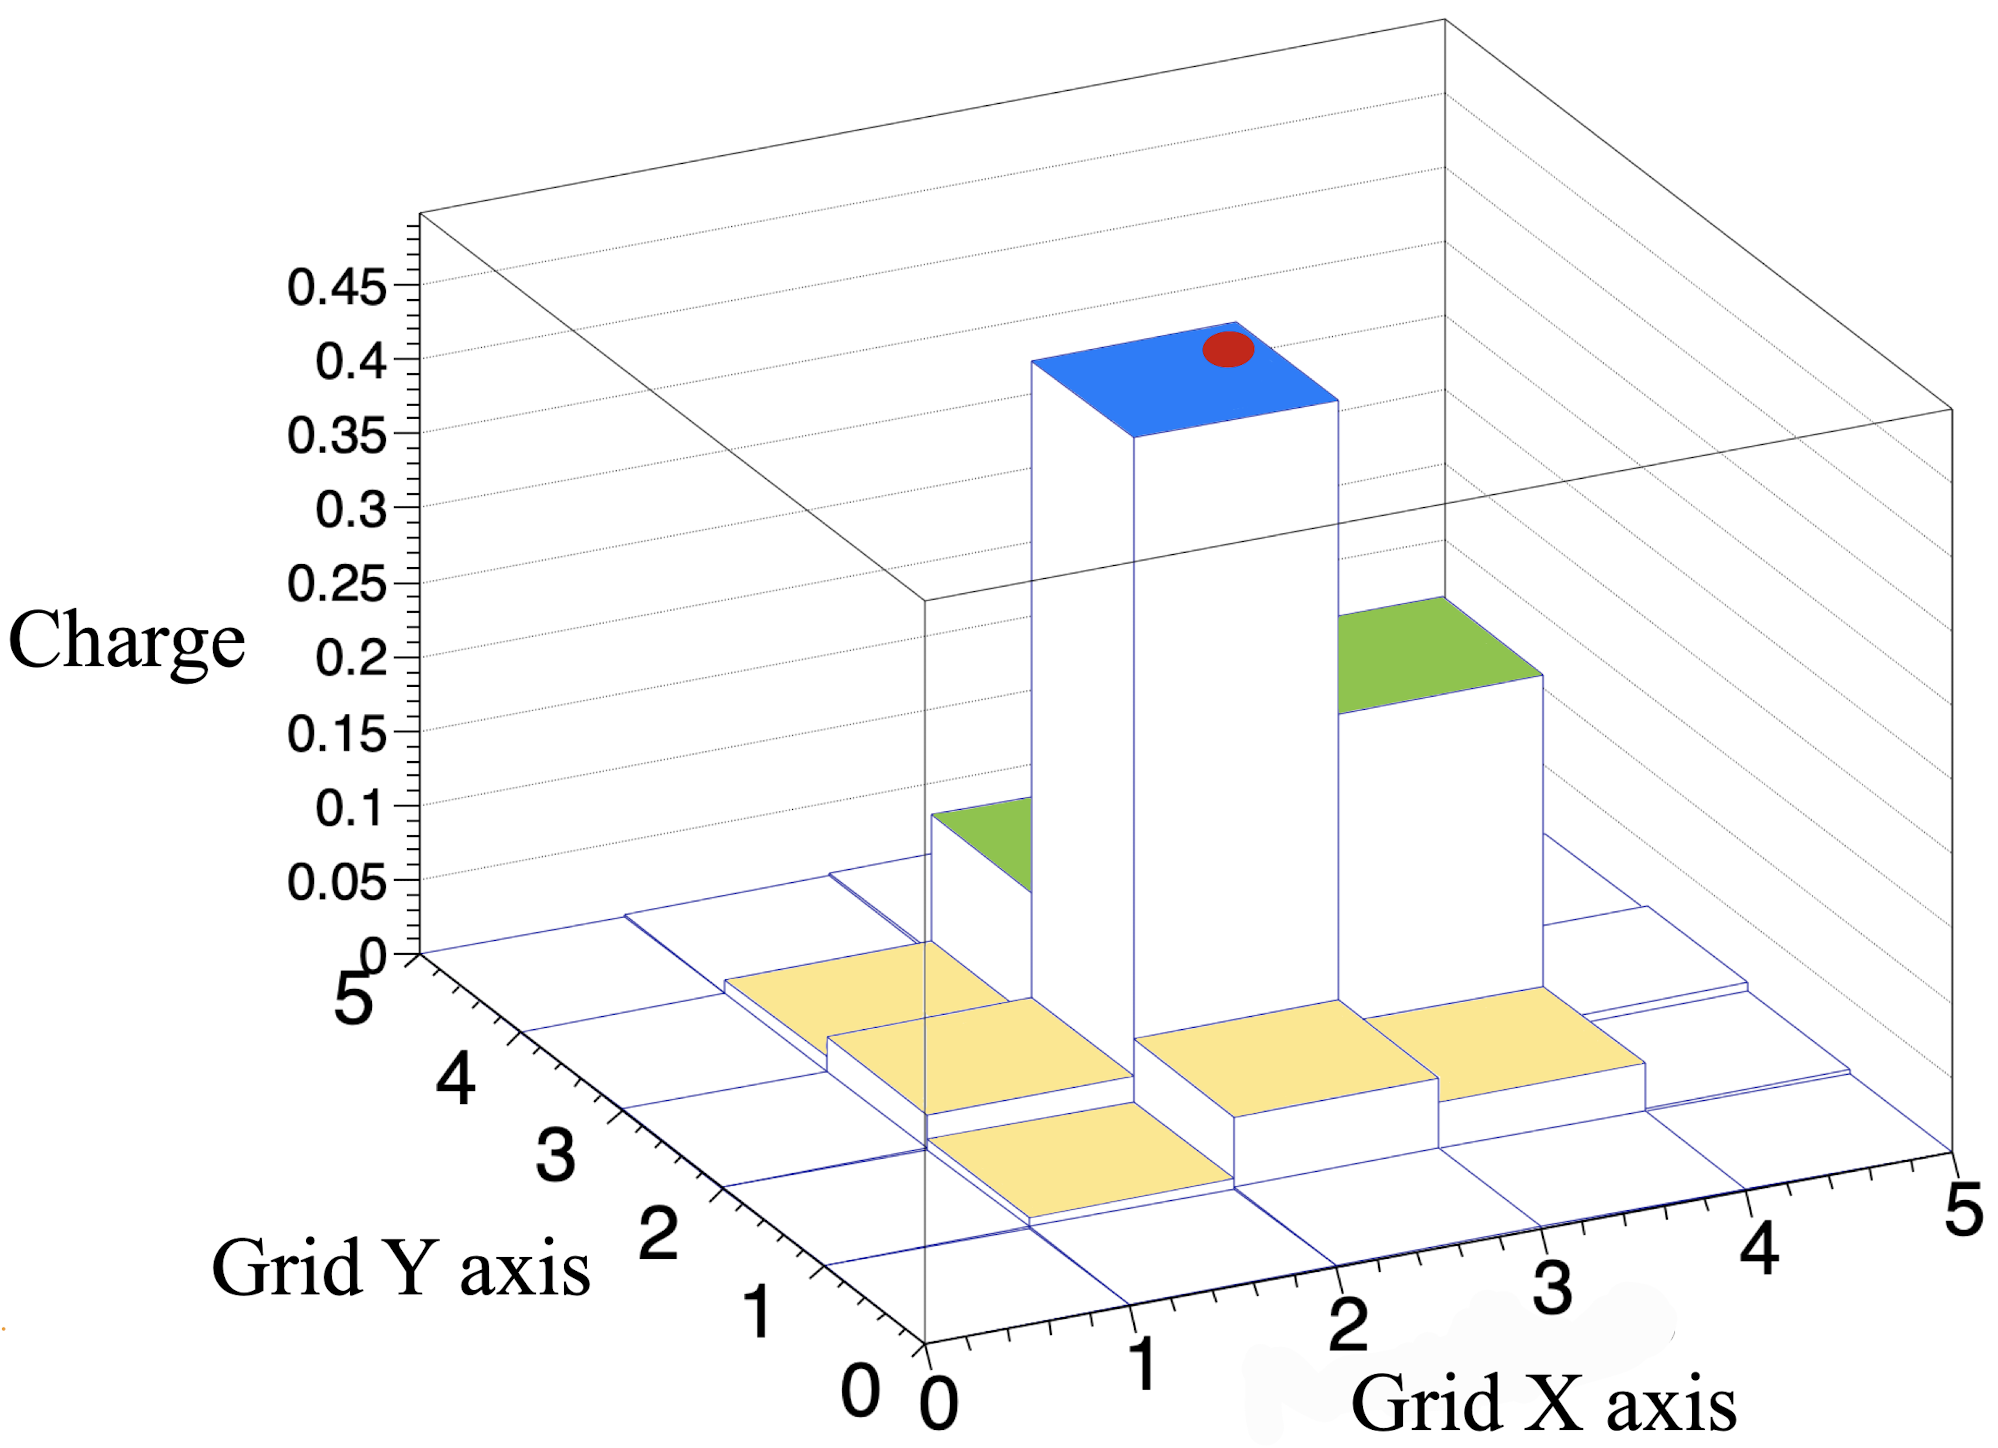
\includegraphics[width=0.7\linewidth]{images/charge_distribution.png}
        \caption{Charge distribution for the original x-ray coordinate $x=2.9$ and $y=2.7$.}
        \label{fig:charge}
    \end{figure}

    We can intuitively see which pixel the x-ray hit. The x-ray hit the pixel in the middle of the grid at the position $x=2$ and $y=2$ because this pixel accumulated the most charge. We can also tell that the x-ray hit the middle pixel at the upper right corner by looking at the neighboring pixels. We can see that the green neighboring pixels on the right accumulated more charge than the yellow pixels on the left. Therefore, the x-ray hit the pixel at a position that is closer to the green pixels than the yellow pixels. Based on this reasoning, we can guess that the original coordinate is approximately where the red dot is.

    \heading{The Model}

    In order to formally predict the original x-ray coordinate, we need to fit a model to our charge distribution. We have chosen two-dimensional Gaussian model which is defined by five parameters - the height of its peak, $x$ and $y$ coordinates of its peak, and the width of the bell in the $x$ and $y$ direction. The position of the peak is an estimate of the original x-ray coordinate because the peak accumulated the most charge.

  \end{block}


\end{column}

\separatorcolumn

\begin{column}{\colwidth}
    \vspace{2.2cm}
    
    In Figure \ref{fig:model}, we can see the mathematically computed and predicted charge distribution. The position of the predicted peak is $x=2.872$ and $y=2.673$ which is very close to the original x-ray coordinate which is $x=2.9$ and $y=2.7$. Furthermore, in Figure \ref{fig:model}, we can see that our model has very low prediction errors (less than 20\%) around the middle pixel where the x-ray hit. Therefore, we can see that our model is accurate in this case.
    \vspace{0.8cm}

    \begin{figure}[H]
    \centering
    \begin{subfigure}{.5\textwidth}
      \centering
      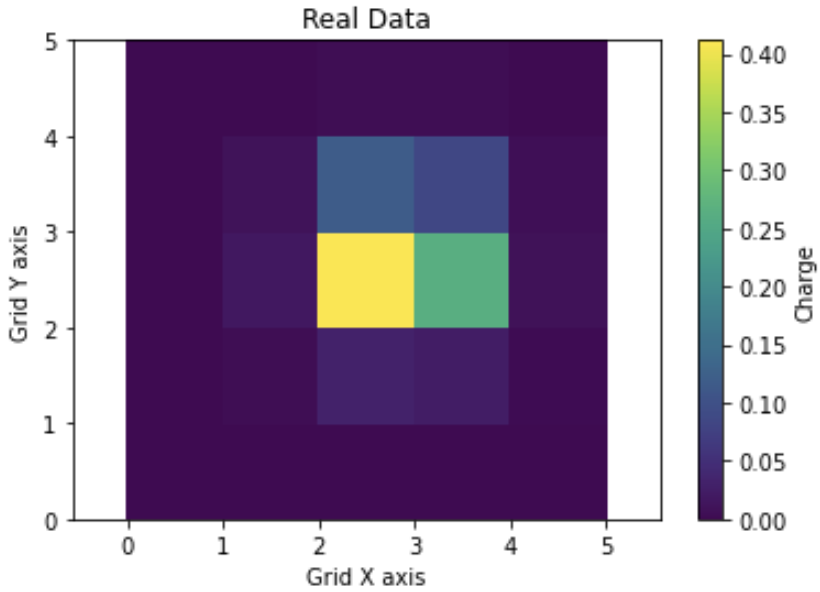
\includegraphics[width=1\linewidth]{images/real.png}
      \caption{Charge distribution computed by the formula}
      \label{fig:sub1}
    \end{subfigure}%
    \begin{subfigure}{.5\textwidth}
      \centering
      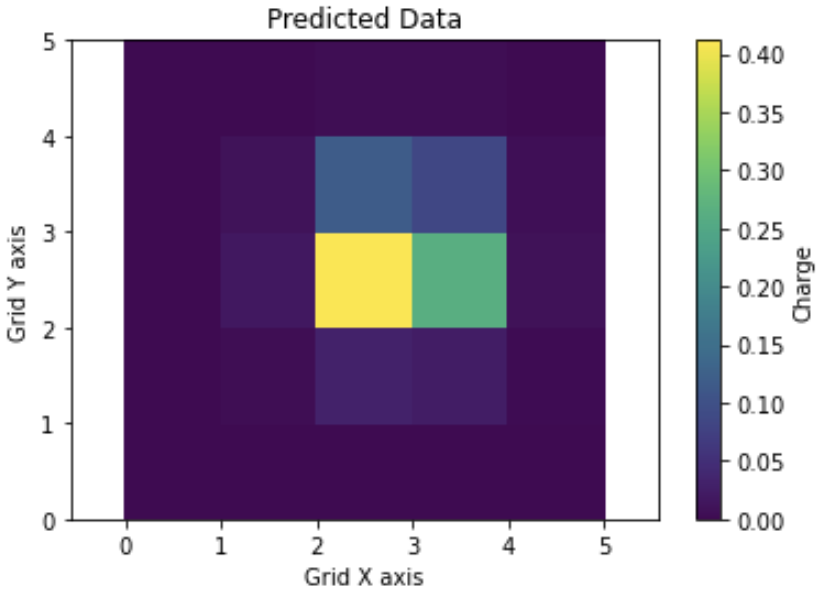
\includegraphics[width=1\linewidth]{images/predicted.png}
      \caption{Charge distribution predicted by the model}
      \label{fig:sub2}
    \end{subfigure}
    \caption{Charge distributions}
    \label{fig:model}
    \end{figure}

    \heading{The Accuracy of the Model}
    \vspace{0.5cm}

    As we can see from the Figure \ref{fig:model}, the two-dimensional Gaussian model is very accurate. The prediction error rate ranges from 0 to 0.6 pixel pitch and most of the errors are less than 0.1 pixel pitch. 
    \vspace{0.8cm}

    \begin{figure}[H]
    \centering
    \begin{subfigure}{.5\textwidth}
      \centering
      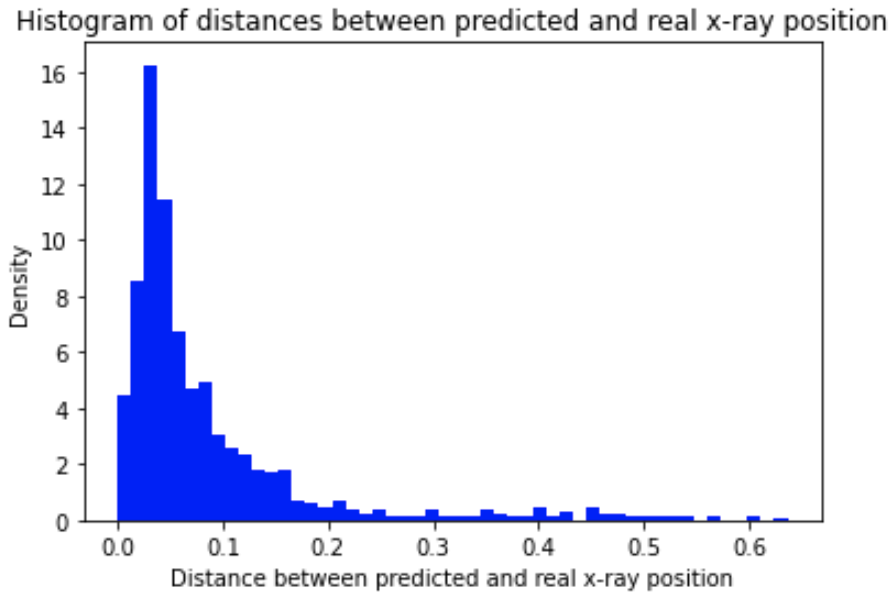
\includegraphics[width=1\linewidth]{images/histogram.png}
      \caption{Histogram of distances}
      \label{fig:sub1}
    \end{subfigure}%
    \begin{subfigure}{.5\textwidth}
      \centering
      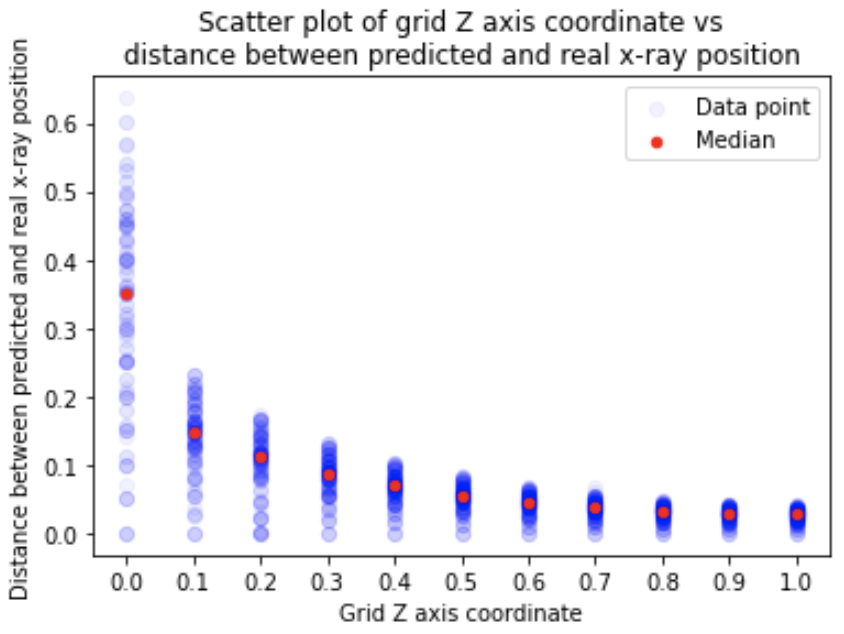
\includegraphics[width=0.9\linewidth]{images/scatter_plot.png}
      \caption{Scatter plot of distances}
      \label{fig:sub2}
    \end{subfigure}
    \caption{The accuracy of the model}
    \label{fig:model}
    \end{figure}


  \begin{block}{Conclusion}
    We have developed a C++ program that takes the x-ray coordinate and outputs its theoretical charge distribution over the $5\times 5$ pixel grid. We have also developed a two-dimensional Gaussian model that predicts the x-ray coordinate given a charge distribution. This model is accurate because it can predict the x-ray coordinate with a very low error rate.\\
    Our project will empower other scientists who come to Brookhaven National Laboratory to explore structures of various materials.
    

  \end{block}


\end{column}

\separatorcolumn
\end{columns}
\end{frame}

\end{document}
